\section{Introduction}

Dynamic languages are increasingly popular etc. etc.

The easiest way to implement a dynamic language such as Python is to write an
interpreter; however, interpreters are slow.

The alternative is to write a compiler; writing a compiler that targets a high
level virtual machine like CLI or JVM is easier than targeting a real CPU, but
it still require a lot of work, as IronPython, Jython, JRuby demonstrate.

Moreover, writing a static compiler is often not enough to get high
performances; IronPython and JRuby are going in the direction of JIT compiling
specialized versions of the code depending on the actual values/types seen at
runtime; this approach seems to work, but write it manually requires an
enormous effort.

PyPy's idea is to automatize the generation of static/JIT compilers in order
to reduce at minimun the effort required to get a fast implementation of a
dynamic language; all you have to do is to write a high level specification of
the language (by writing an interpreter), and put it through PyPy's
translation toolchain.

\subsection{PyPy and RPython}

\anto{as Armin points out, the two CLI backends can be easily confused; what
  about renaming the ``CLI Backend for flowgraphs'' into ``CLI bytecode
  compiler''? Any better idea for the name?}

\begin{figure}[h]
\begin{center}
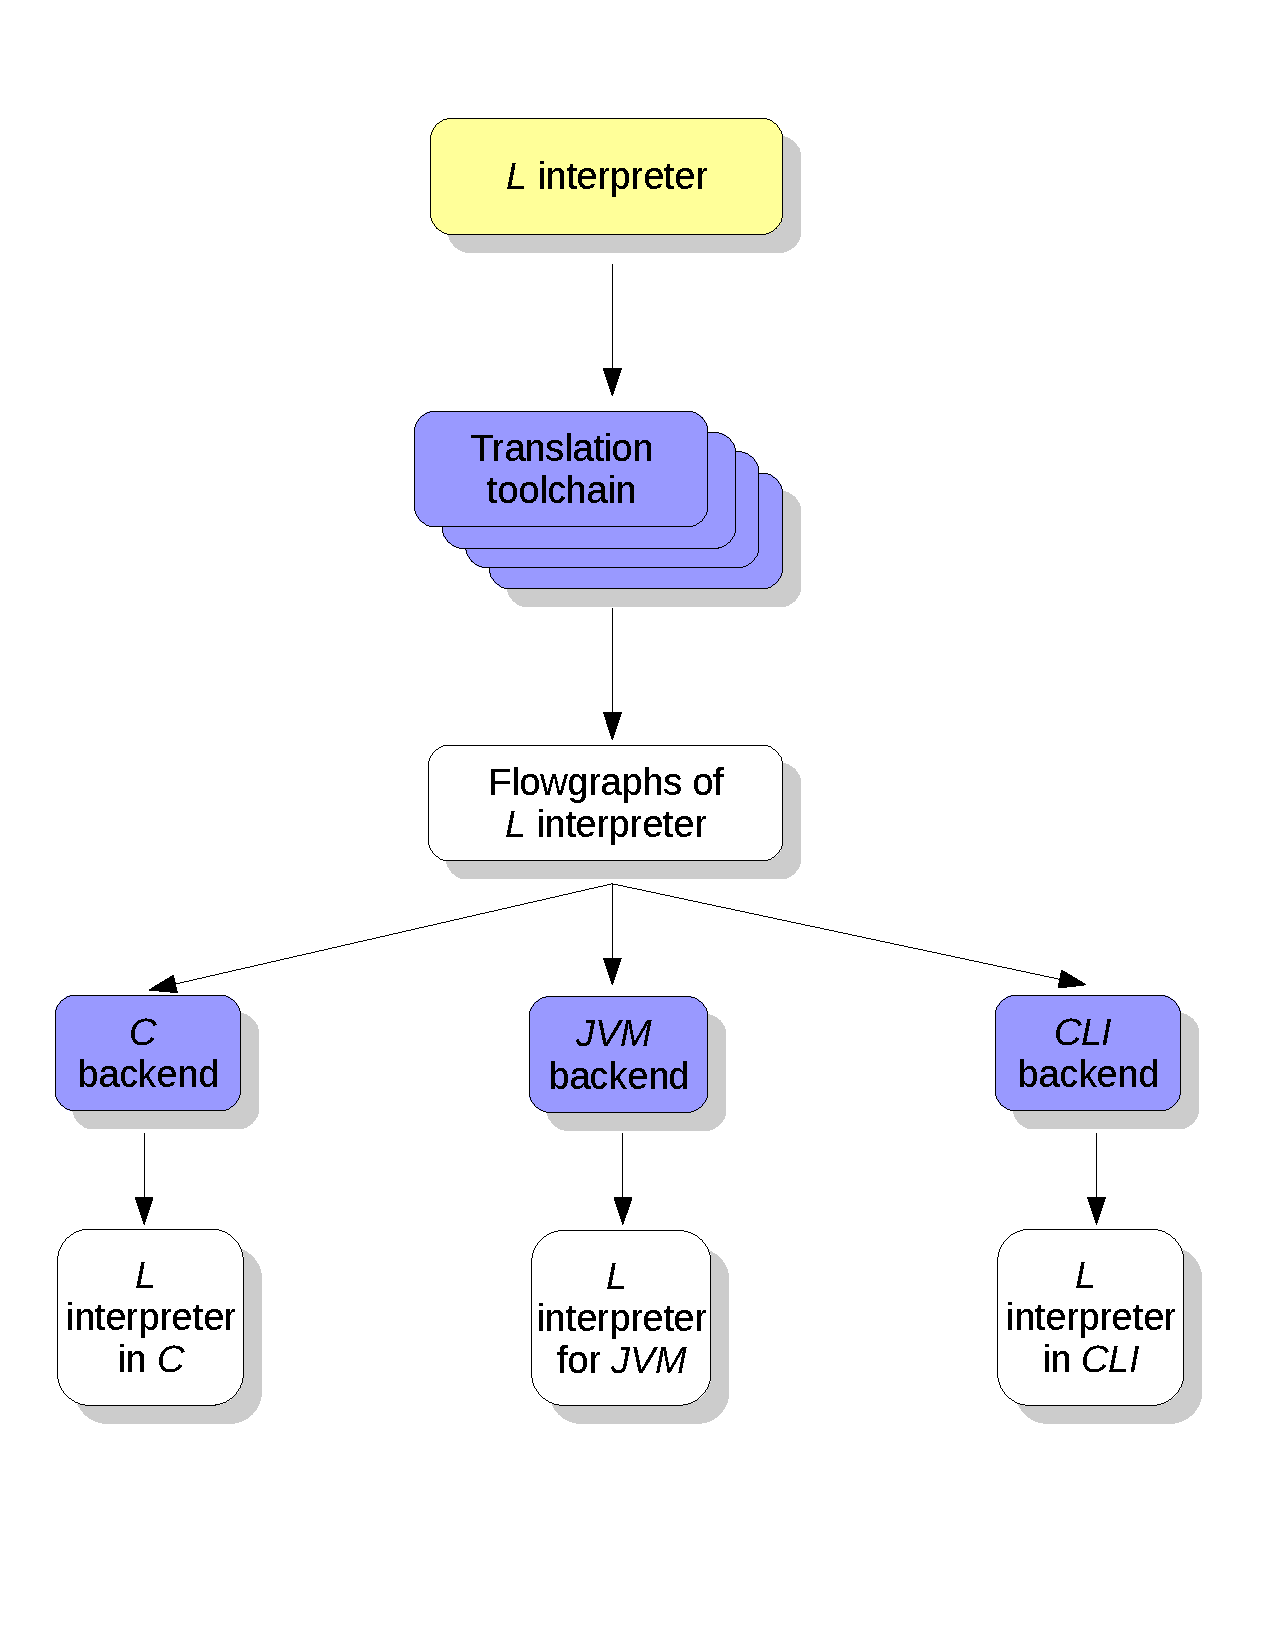
\includegraphics[width=.6\textwidth]{diagram0}
\caption{PyPy infrastracture for generating an interpreter of a
  language $L$ for several platforms}\label{pypy-fig}
\end{center}
\end{figure}

The \emph{PyPy} project\footnote{\texttt{http://codespeak.net/pypy/dist/pypy/doc/home.html}}
\cite{RigoPedroni06} was initially conceived to develop an implementation of Python which
could be easily portable and extensible without renouncing efficiency.
To achieve these aims, the PyPy implementation is based on a highly
modular design which allows high-level aspects
to be separated from lower-level implementation details.
The abstract semantics of Python is defined by an interpreter written
in a high-level language, called RPython \cite{AACM-DLS07}, which is in fact a subset of
Python where some dynamic features have been sacrificed to allow an
efficient translation of the interpreter to low-level code.

Compilation of the interpreter is implemented as a stepwise
refinement by means of a translation toolchain which performs type
analysis, code optimizations and several transformations aiming at 
incrementally providing implementation details as memory management or the threading model.
The different kinds of intermediate codes  which are refined 
during the translation process are all represented by a collection of control flow graphs,
at several levels of abstractions.

Finally, the low-level control flow-graphs produced by the toolchain
can be translated to executable code for a specific platform by a
corresponding backend.
Currently, three fully developed backends are available to produce
executable C/POSIX code, Java and CLI/.NET bytecode. 

Despite the PyPy infrastructure was specifically developed 
for Python, in fact it can be used for implementing
other languages. Indeed, PyPy has been successfully experimented with
several languages as Smalltalk \cite{BolzEtAl08}, JavaScript, Scheme and Prolog.
As suggested by Figure~\ref{pypy-fig}, a portable interpreter for a
generic language $L$  can be
easily developed once an abstract interpreter for $L$ is implemented in
RPython.

Another interesting feature of PyPy
is that just-in-time compilers can be semi-automatically generated from the
interpreter source.
